\section{Ausgangssituation}\label{sec:introduction}

Es gibt bereits viele VR Applikation, aber was ist genau eine VR Applikation.
Es gibt viele Definition für VR ausgeschrieben Virtual Reality.
In dieser Arbeit sprechen wir über die Wirklichkeit welche durch ein head mounted display, oder umagangssprachlich auch eine VR-Brillge angezeigt wird.
Somit bezeichnet eine VR Applikationn eine Software welche in der VR-Brille läuft.

Von diesen VR Applikationen gibt es schon einige.
Die meisten werden im Bereich Videospiele verwendet nach einer Statistik aus Deutschland im Jahre 2021.

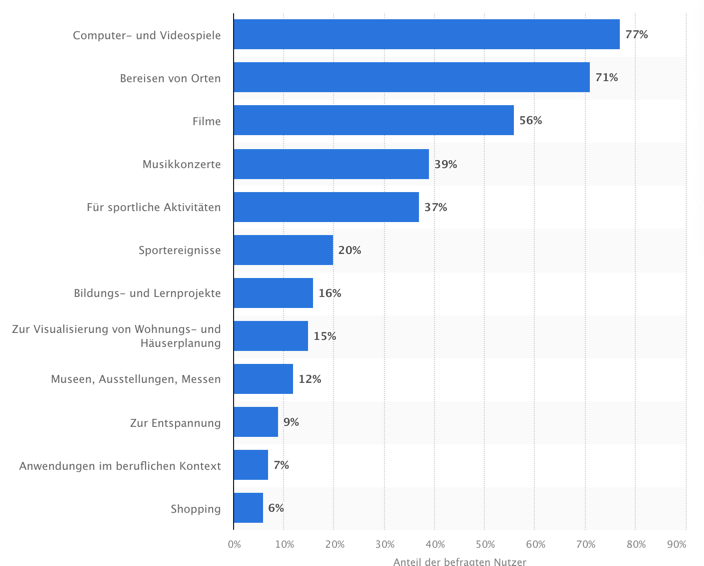
\includegraphics[scale=0.5]{pics/statistic_anwendungsgebiete_vr}



BeamVR ist ein Projekt, welches das Ziel verfolgt die virtuelle und physische Realität zu kombinieren,
um eine höhere Immersion zu erzielen.
Der virtuelle baleen steht von einem Hochhaus ab, während der physische Balken auf vertrauten Grund liegt.
Das Programm synchronisiert dabei einen Balken welcher in der virtuellen und physischen Realität vorhanden ist.
Durch die Synchronisierung soll einem das Gefühl gegeben werden, dass er wirklich auf einem Balken steht, welcher von
einem Hochhaus absteht.

Beam VR ist aber nicht der Erfinder dieses Konzeptes, was in der kommenden Umfeldanalyse gezeigt wird.

\section{Zielsetzung}\label{sec:objective}
